\documentclass[border=20pt]{standalone}
\usepackage{tikz}
\usetikzlibrary{positioning,arrows.meta}
\begin{document}
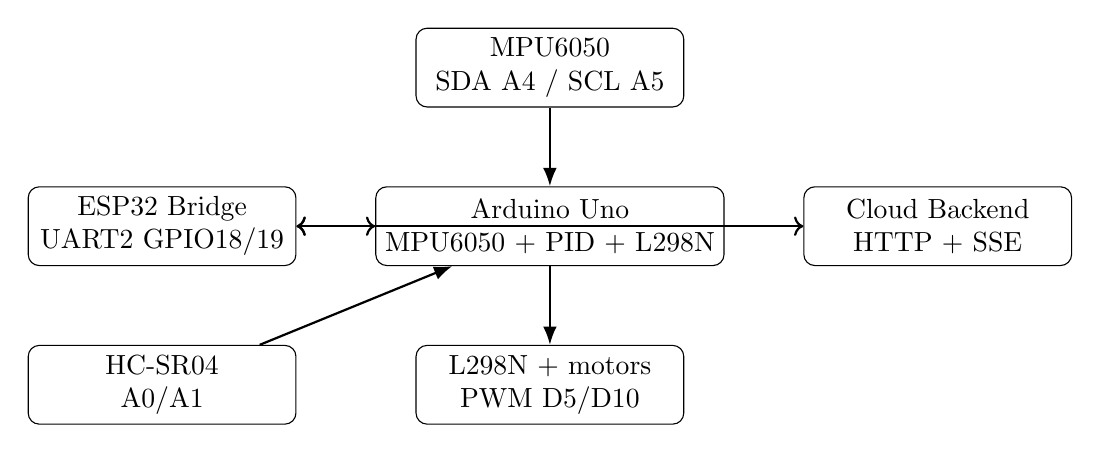
\begin{tikzpicture}[node/.style={draw,rounded corners,align=center,minimum width=3.4cm,minimum height=1cm},line/.style={-Latex,thick}]
\node[node] (a) {Arduino Uno\\MPU6050 + PID + L298N};
\node[node,above=of a] (m) {MPU6050\\SDA A4 / SCL A5};
\node[node,below=of a] (d) {L298N + motors\\PWM D5/D10};
\node[node,left=of a] (e) {ESP32 Bridge\\UART2 GPIO18/19};
\node[node,right=of a] (c) {Cloud Backend\\HTTP + SSE};
\node[node,below left=of a] (s) {HC-SR04\\A0/A1};
\draw[line] (m)--(a);\draw[line] (a)--(d);\draw[line,<->] (e)--(a);\draw[line,<->] (e)--(c);\draw[line] (s)--(a);
\end{tikzpicture}
\end{document}
